Giving a step input to a high-gain PID position controlled actuator can cause an over current fault, burn out motor drivers, strip gears due to the \textit{jerk} etc.  
To reduce this effect Hubo-Ach has multiple modes of on-board filtering.
These modes are:
\begin{itemize}
\item Reference Input Filtering
\item Compliance Amplification 
\end{itemize}

This section talks about \textit{reference input filtering} as a method to apply a step input each joint in joint space and limit the jerk.
It is important to note that the obvious answer is to reduce the PID gains to make the robot \textit{more complaint} however the goal of this work is to make a fully functional system that does not require modification of the robot.
In this case the PID gains are set by the motor drivers and that is considered to be a part of the robot.
In future firmware updates of the motor drivers we will have the ability to change PID gains on the fly.

\textit{reference input filtering} uses the history of the previous $\theta_c$ sent to the given actuator.  The current commanded actuator position $\theta_c(N)$ is given by:

\begin{equation}\label{eq:reffiltermode}
\theta_c(N) = \frac{\theta_c(N-1)\cdot\left(L-1\right) + \theta_r(N)}{L}
\end{equation}

Where $L$ is an integer that represents the length of the filter and $L\geq1$.  
If $L=1$ then Equation~\ref{eq:reffiltermode} becomes Equation~\ref{eq:refrefmode}.

\begin{figure}
\centering

\begin{tikzpicture}[->,>=stealth',shorten >=1pt,auto,node distance=5cm,
  thick,main node/.style={fill=white!20,draw,font=\sffamily\Large\bfseries}]


  \node[main node] (ref) {Reference};
  \node[main node] (filter) [right=3.0cm of ref] {Filter};
  \node[main node] (hubo-ach) [below=1.0cm of filter] {Hubo-Ach};
  \node[main node] (hubo) [right=3.0cm of hubo-ach] {Hubo};




  \path[<->,dashed, every node/.style={font=\sffamily\small}]
    (hubo) edge node [above] {CAN} (hubo-ach);

  \path[->,every node/.style={font=\sffamily\small}]
    (ref) edge node [above] {$\theta_d$} (filter);

  \path[->,every node/.style={font=\sffamily\small}]
    (filter) edge node [left] {$\theta_r$} (hubo-ach);


\end{tikzpicture}
\caption{Desired reference $\theta_d$ being filtered before applied to Hubo via Hubo-Ach.  $\theta_d$ is sent through a filter that reduces the \textit{jerk} on the actuator then the new reference $\theta_r$ is set on the \textbf{FeedForward} channel, Hubo-Ach reads it then commands Hubo at the rising edge of the next cycle.}
\label{fig:hubo-ach-feedforward}
\end{figure}





Fig.~\ref{fig:singleJointStepFiltered} shows the commanded reference plotted again the actual reference using the filtered mode defined in Equation~\ref{eq:reffiltermode}.
Fig.~\ref{fig:singleJointStepFilteredLtest} shows the $\theta_r$ plotted against $\theta_c$ and $\theta_a$ for different values of $L$.
It is easy to see that as $L$ increases the $t_{rise}$ also increases and the \textit{jerk} is reduced.


\begin{figure}[thpb]
  \centering
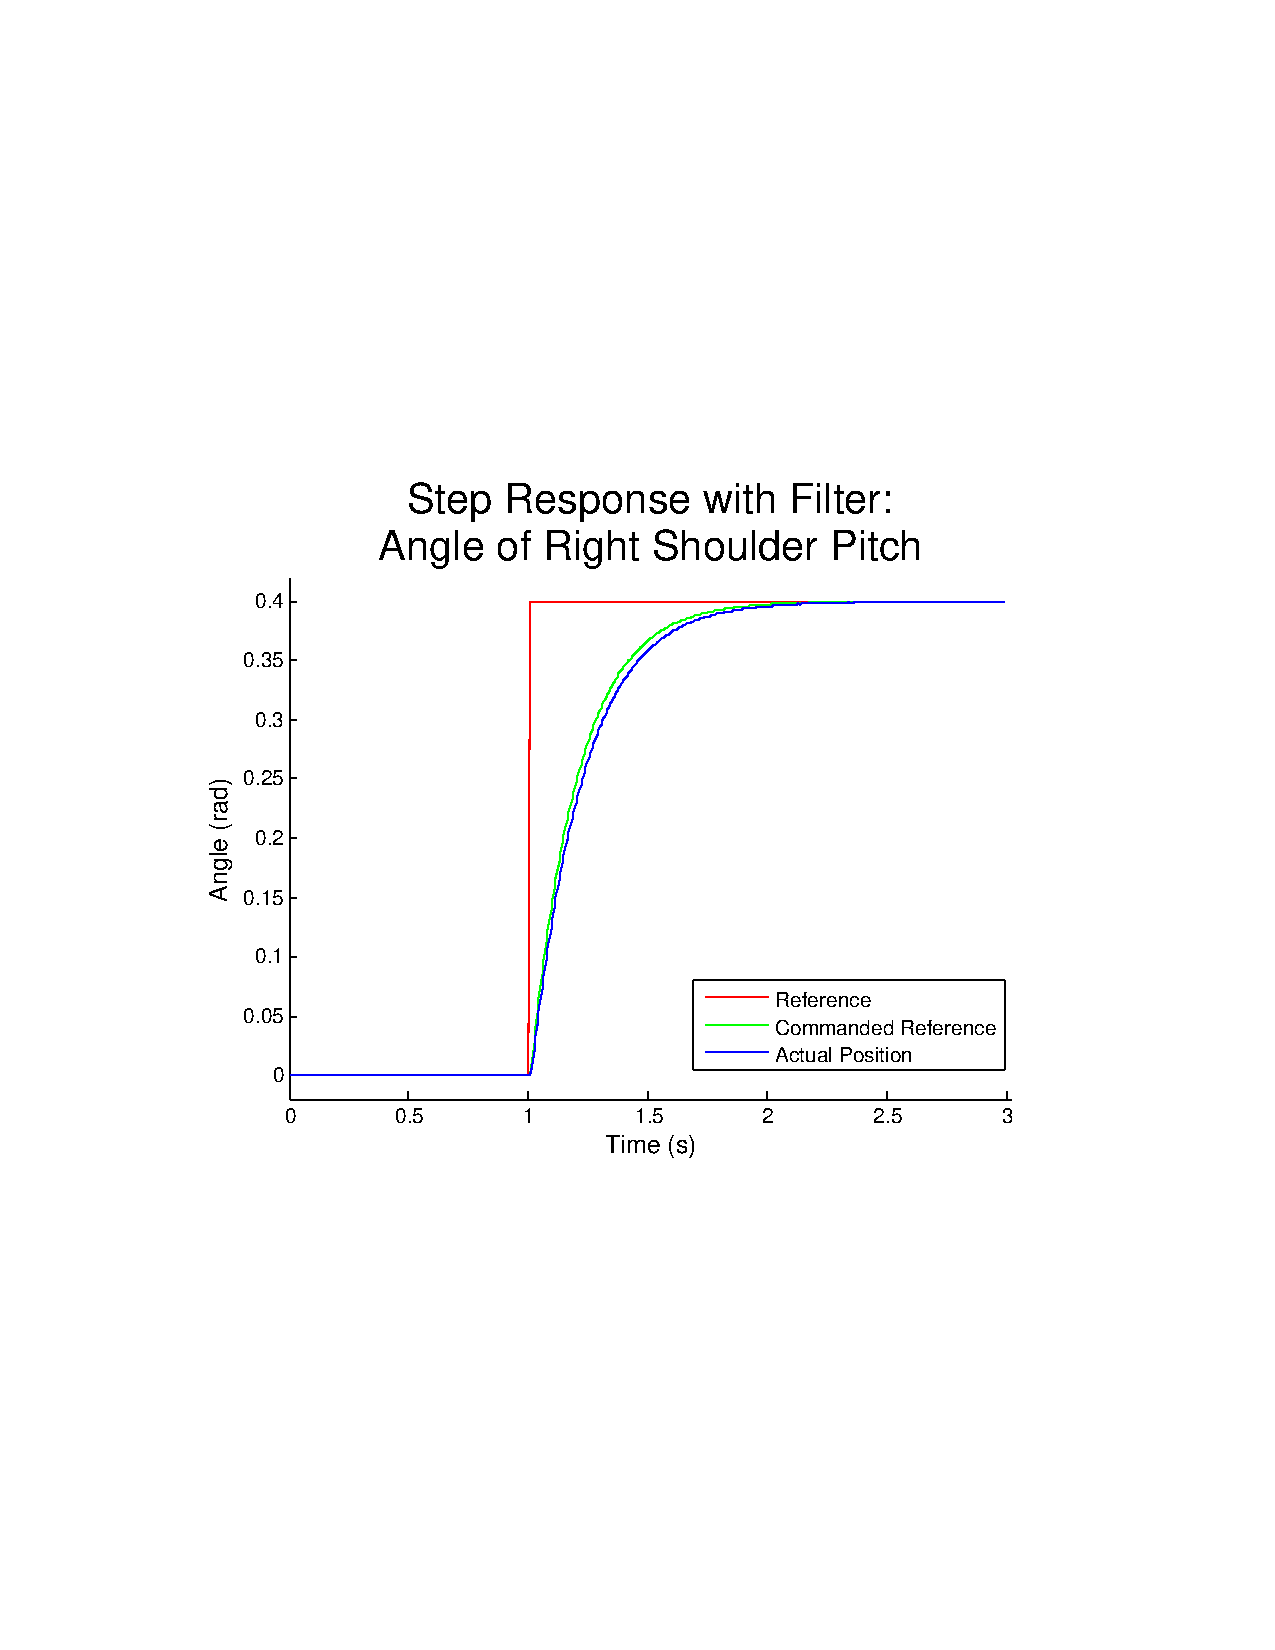
\includegraphics[width=0.8\columnwidth]{./examples/pix/RSP-Zp4-step-filter-crop.pdf}
  \caption{The commanded reference plotted against the actual reference recorded  In this plot the commanded reference is automatically filtered by Hubo-Ach.}
%\caption{The commanded reference plotted against the actual reference recorded via Hubo-Ach and ground truth via CAN analyzing utilities.  In this plot the commanded reference is automatically filtered by Hubo-Ach.}
  \label{fig:singleJointStepFiltered}
\end{figure}

\begin{figure}[thpb]
  \centering
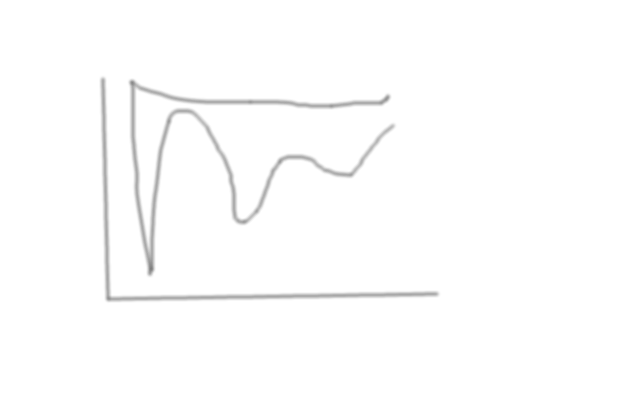
\includegraphics[width=0.8\columnwidth]{./pix/tmp.png}
  \caption{$\theta_r$ plotted against $\theta_c$ and $\theta_a$ recorded via Hubo-Ach with values for $L$ ranging from 1 to 200.}
  \label{fig:singleJointStepFilteredLtest}
\end{figure}

This method is a feed-forward method that assumes that the position you set the actuator to is the actual position of the actuator.
